% \begin{figure}[t]
%     \centering
%     % Four independent panels, each generated by its own Python script
%     % under unified style (see ICML2026-submission-figure-script-drawio-todo/wandb-figure/).
%     \begin{minipage}[t]{0.245\linewidth}
%         \centering
%         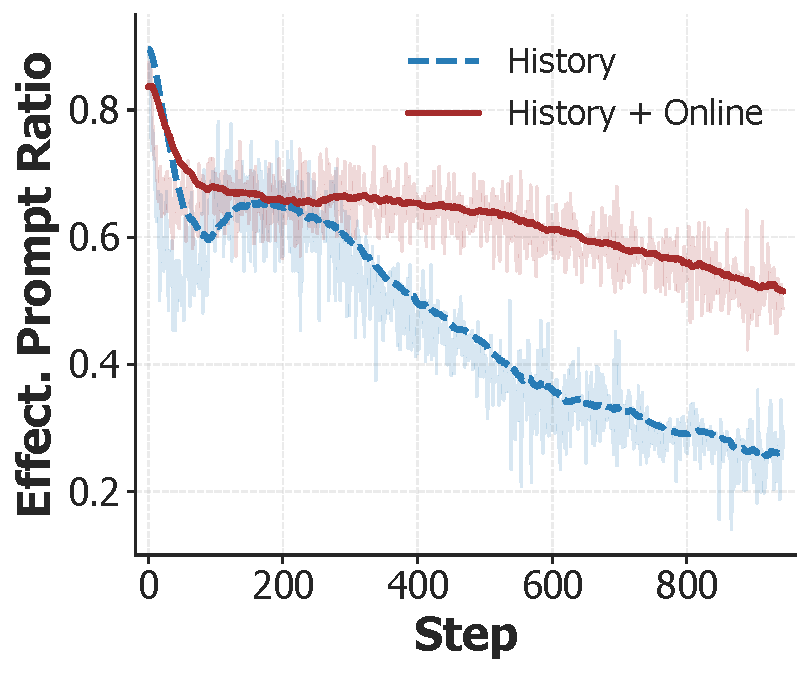
\includegraphics[width=\linewidth]{figures/intro/intro_a_eff_ratio.pdf}
%         \\[-2pt]{\footnotesize\textbf{(a)}\par}
%     \end{minipage}\hfill
%     \begin{minipage}[t]{0.245\linewidth}
%         \centering
%         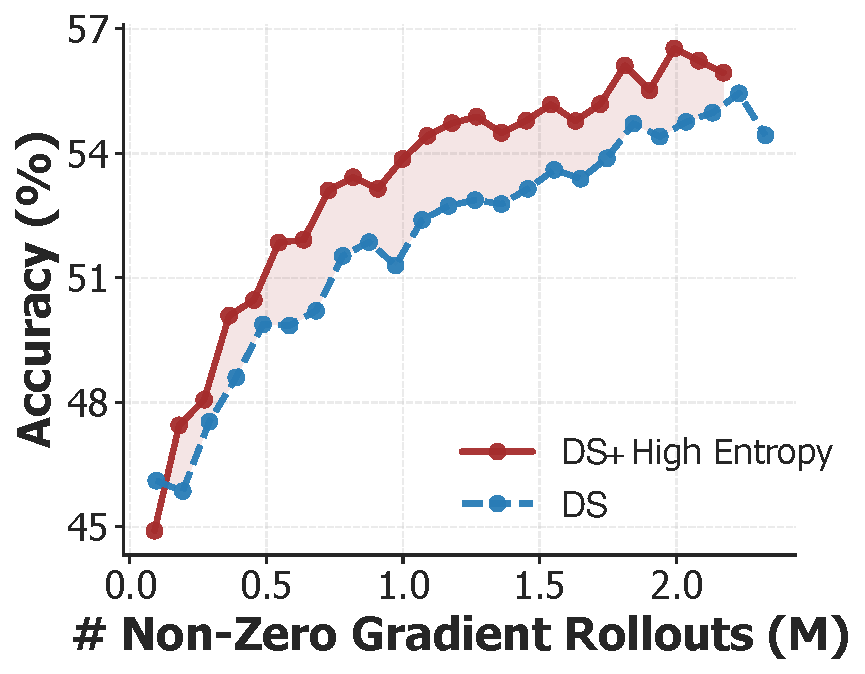
\includegraphics[width=\linewidth]{figures/intro/intro_b_high_entropy-backup.pdf}
%         \\[-2pt]{\footnotesize\textbf{(b)}\par}
%     \end{minipage}\hfill
%     \begin{minipage}[t]{0.245\linewidth}
%         \centering
%         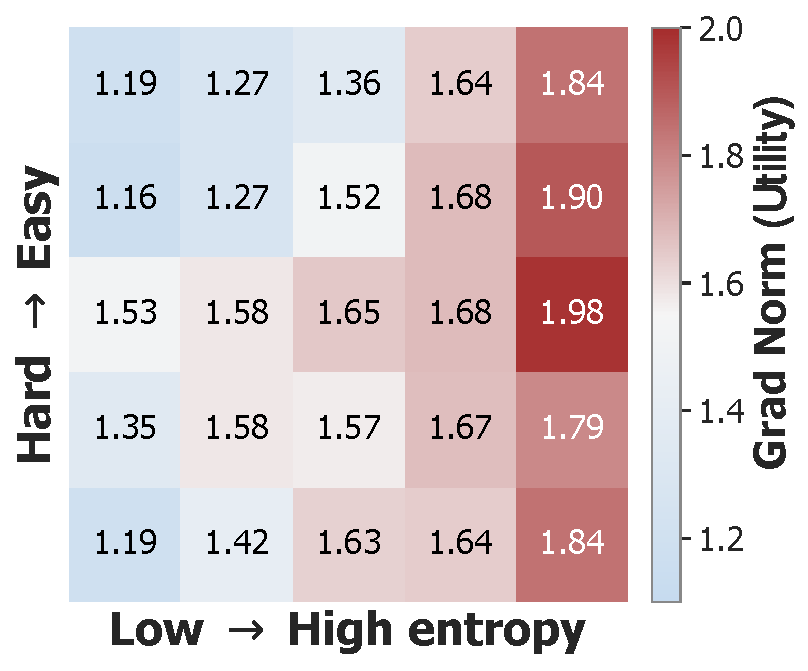
\includegraphics[width=\linewidth]{figures/intro/intro_c_heatmap-backup.pdf}
%         \\[-2pt]{\footnotesize\textbf{(c)}\par}
%     \end{minipage}\hfill
%     \begin{minipage}[t]{0.245\linewidth}
%         \centering
%         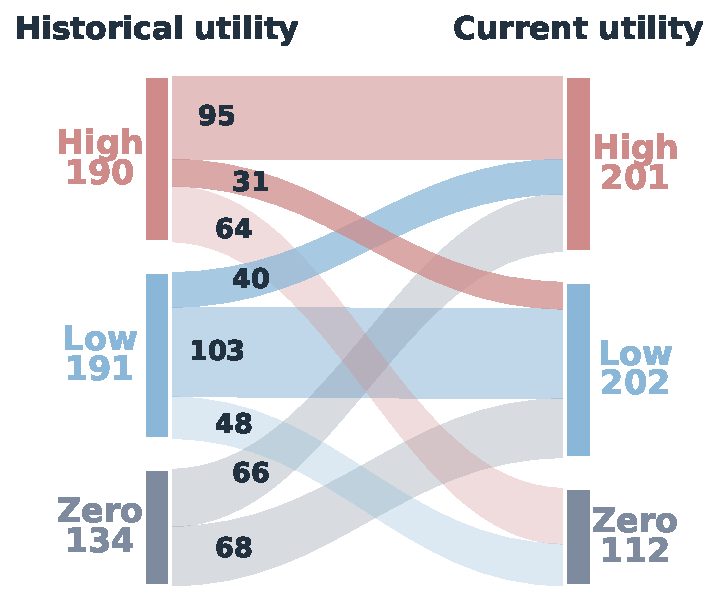
\includegraphics[width=\linewidth]{figures/intro/intro_d_sankey.pdf}
%         \\[-2pt]{\footnotesize\textbf{(d)}\par}
%     \end{minipage}
%     \caption{\textbf{Four empirical observations motivating HIVE.}
%     (a) Selection only based on historical statistics becomes increasingly stale during training, while online verification retains more effective prompts.
%     (b) Among prompts with non-zero gradients, prioritizing high-entropy
%         prompts improves accuracy at the same rollout budget.
%     (c) Gradient utility concentrates at an intermediate-difficulty,
%         high-entropy learning edge.
%     (d) Across two checkpoints (steps 500 and 1000), a large fraction of sampled
%         prompts shift between High, Low, and Zero utility classes, so
%         prompts selected by historical metadata no longer match the
%         current policy's utility distribution. \red{(1) need to re-write the corresponding prelimiary analysis and (2) revise the reference of these four subfigures.}
%     }
%     \label{fig:intro-a-b}
%     \vskip -0.15in
% \end{figure}
\begin{figure}[t]
    \centering
    \captionsetup[subfigure]{labelformat=parens,labelsep=none,font=footnotesize,justification=centering}
    % Four independent panels, each generated by its own Python script
    % under unified style (see ICML2026-submission-figure-script-drawio-todo/wandb-figure/).
    \begin{subfigure}[t]{0.241\linewidth}
        \centering
        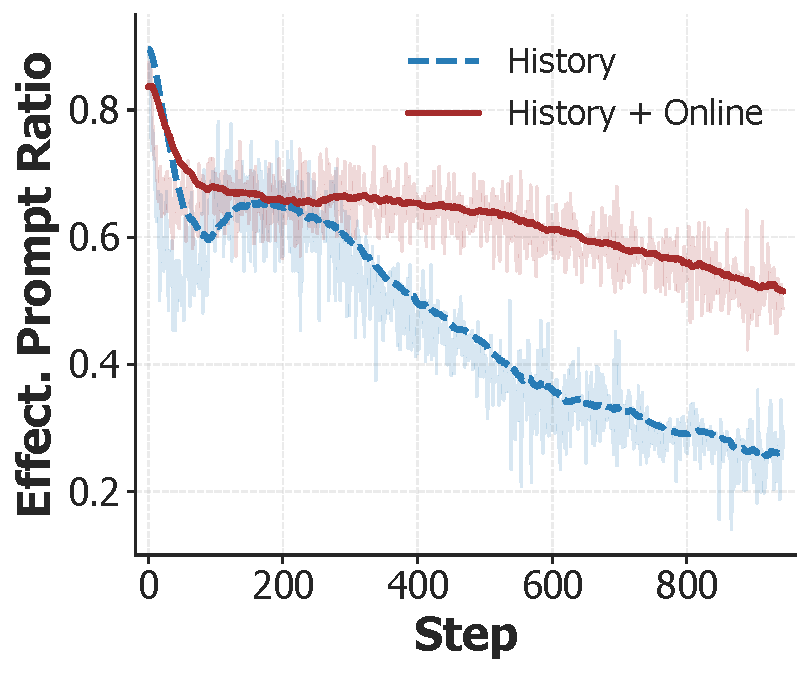
\includegraphics[width=\linewidth]{figures/intro/intro_a_eff_ratio.pdf}
        \vspace{-6pt}
        \caption{}
        \label{fig:intro-history-staleness}
    \end{subfigure}\hfill
    \begin{subfigure}[t]{0.245\linewidth}
        \centering
        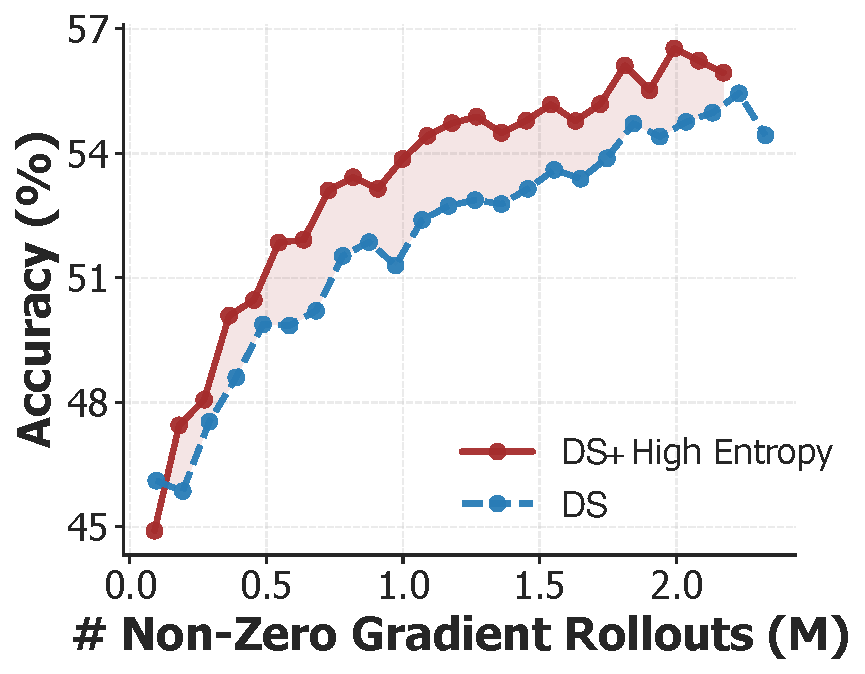
\includegraphics[width=\linewidth]{figures/intro/intro_b_high_entropy-backup.pdf}
        \vspace{-6pt}
        \caption{}
        \label{fig:intro-high-entropy}
    \end{subfigure}\hfill
    \begin{subfigure}[t]{0.245\linewidth}
        \centering
        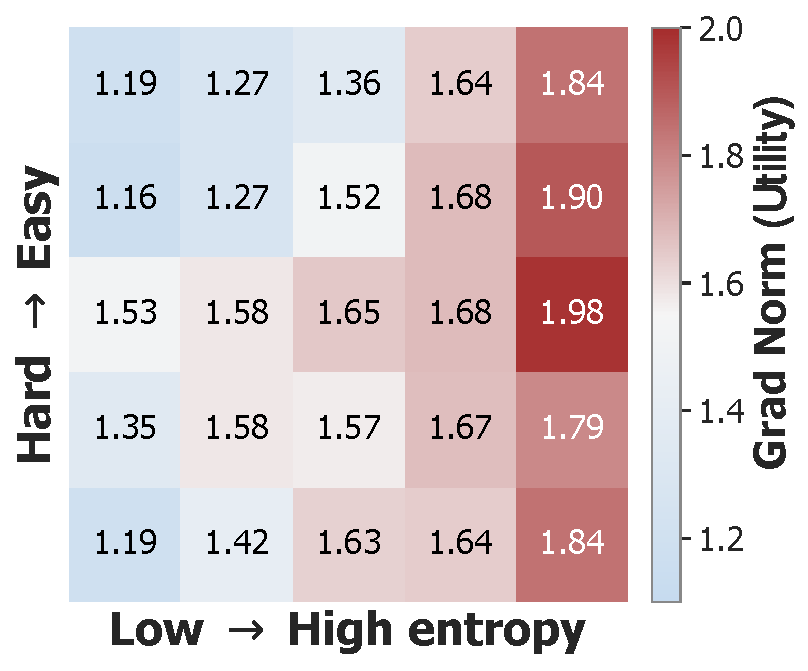
\includegraphics[width=\linewidth]{figures/intro/intro_c_heatmap-backup.pdf}
        \vspace{-6pt}
        \caption{}
        \label{fig:intro-learning-edge}
    \end{subfigure}\hfill
    \begin{subfigure}[t]{0.241\linewidth}
        \centering
        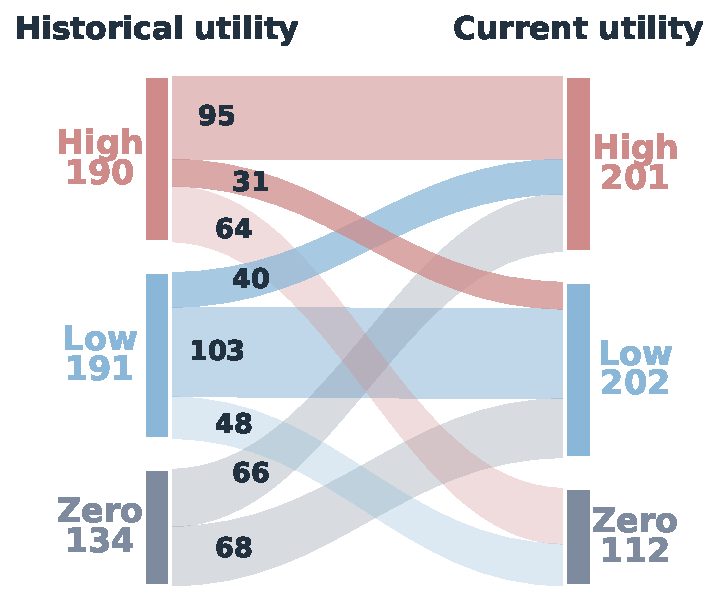
\includegraphics[width=\linewidth]{figures/intro/intro_d_sankey.pdf}
        \vspace{-6pt}
        \caption{}
        \label{fig:intro-utility-shift}
    \end{subfigure}
    \caption{\textbf{Empirical observations.}
    (a) Selection only based on historical statistics becomes increasingly stale during training, while online verification retains more effective prompts.
    (b) Among prompts with non-zero gradients, prioritizing high-entropy
        prompts improves accuracy at the same rollout budget.
    (c) Gradient utility concentrates at an intermediate-difficulty,
        high-entropy learning edge.
    (d) Across two checkpoints (steps 500 and 1000), a large fraction of sampled
        prompts shift between High, Low, and Zero utility classes, so
        prompts selected by historical metadata no longer match the
        current policy's utility distribution.
    }
    \label{fig:intro-a-b}
    \vskip -0.15in
\end{figure}
